\documentclass[11pt]{article}

\usepackage[margin=2.2cm]{geometry}
\usepackage{amsmath}
\usepackage{listings}
\usepackage{xcolor}
\usepackage{hyperref}
\usepackage{graphicx}
\usepackage{enumitem}
\usepackage{caption}

\hypersetup{colorlinks=true, linkcolor=blue!50!black, urlcolor=blue!50!black}

\lstdefinestyle{py}{
    backgroundcolor=\color{gray!5},
    basicstyle=\ttfamily\footnotesize,
    breaklines=true,
    frame=single,
    rulecolor=\color{gray!40},
    numbers=left,
    numberstyle=\tiny\color{gray!60},
    language=Python,
    tabsize=4,
    columns=fullflexible,
    aboveskip=4pt,
    belowskip=2pt,
}
\lstdefinestyle{sh}{
    backgroundcolor=\color{gray!5},
    basicstyle=\ttfamily\footnotesize,
    breaklines=true,
    frame=single,
    rulecolor=\color{gray!40},
    columns=fullflexible,
    aboveskip=4pt,
    belowskip=2pt,
}
\lstset{style=py}
\captionsetup[lstlisting]{skip=2pt}

\setlength{\parskip}{0.35em}
\setlength{\parindent}{0pt}

\title{OVMM: A Short Tour of \texttt{core/} and \texttt{fetcher}}
\author{}
\date{}

\begin{document}
\sloppy
\maketitle

\section*{Motivation}

Most lab demos of mobile manipulation hard-wire the one task they show: a fixed
object name, a fixed shelf, a fixed grasp, all decided in advance by whoever wrote the
code. That is fine for a demo, but a robot helping in a home, a warehouse, or a
hospital room is asked for things in whatever words the person happens to use, about
objects whose position changes day to day, in a room nobody pre-measured. Closing that
gap is the actual problem here -- not ``can a robot pick up a pringles can'' (easy once
a grasp model exists), but ``can it be told to fetch something in plain language,
guess where that thing probably is from what it has already seen of the room, check,
and adapt if wrong'' -- without anyone hand-coding the object list or the locations in
advance. OVMM is our attempt to build and test that whole loop end to end, in
simulation first, because jumping straight to a polished demo of one isolated stage
hides exactly the integration problems (frame mismatches, timing, bad assumptions
about what the robot already knows) that make the rest of it hard in practice. Below:
a short map of where each piece lives in the code, then a worked integration bug we
hit and fixed.

\section*{Architecture: \texttt{core/} and \texttt{fetcher}}

The project splits into two halves: \texttt{core/} is plain Python with no ROS
dependency (the ``brain''), and the ROS 2 package \texttt{fetcher} is a thin layer that
wires \texttt{core/}'s logic to actual robot topics, services, and actions (the
``body'').

\begin{center}
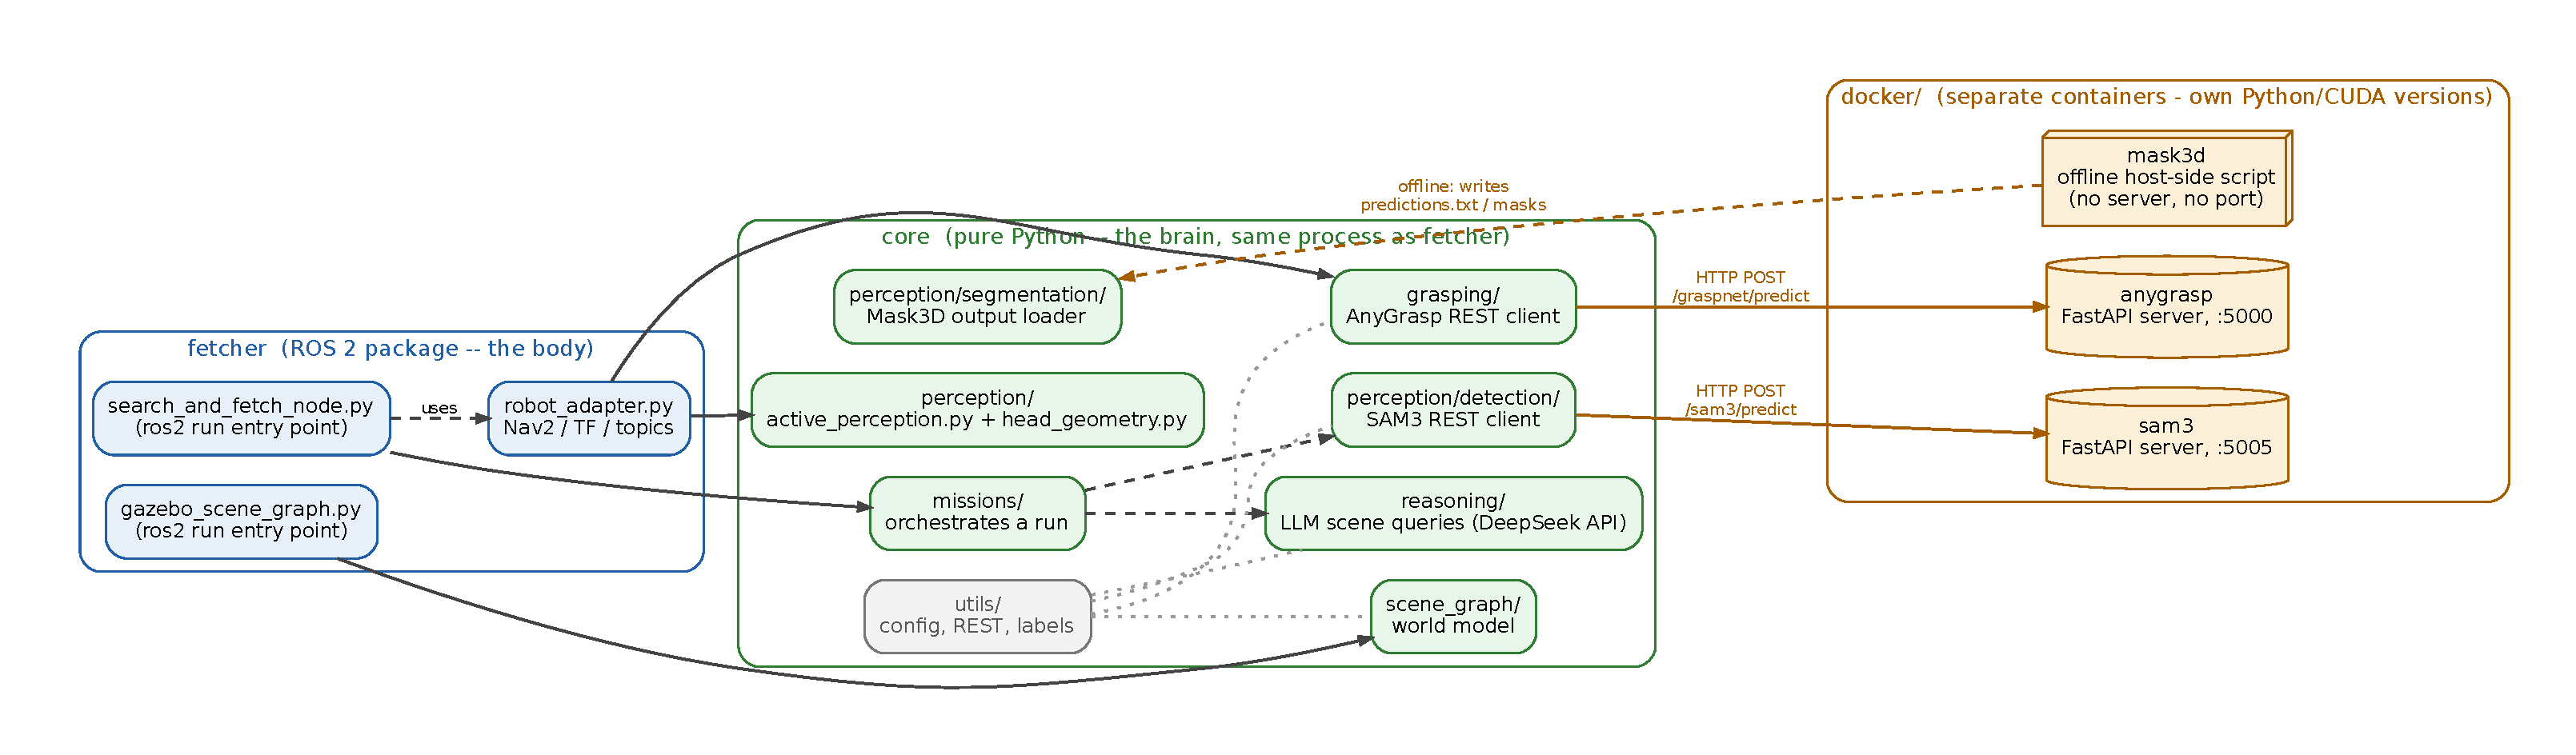
\includegraphics[width=\textwidth]{architecture.pdf}
\end{center}

\begin{description}[itemsep=1pt, topsep=3pt, leftmargin=1.6cm]
  \item[\texttt{perception/}] Sees and aims the camera: SAM3 detection, Mask3D
        loading, and geometry for where to look/stand.
  \item[\texttt{scene\_graph/}] World model -- furniture/objects as nodes (centroid,
        dimensions), connected by ``sits on'' edges.
  \item[\texttt{grasping/}] AnyGrasp REST client: point cloud in, ranked
        collision-aware grasp poses out.
  \item[\texttt{reasoning/}] Talks to the LLM: known-location lookup (Scenario B) or
        top-$k$ furniture prediction when unknown (Scenario A).
  \item[\texttt{missions/}] Orchestrates one fetch (navigate, look, detect, grasp,
        retry) against a \texttt{RobotAdapter} protocol it never implements.
  \item[\texttt{utils/}] Config loading, REST client base class, label tables --
        used by everything above.
\end{description}

\texttt{fetcher} has exactly three files. \texttt{robot\_adapter.py} is the only place
Nav2, TF, camera topics, and joint trajectories appear -- it implements
\texttt{missions}' \texttt{RobotAdapter} protocol for the HSR. The other two are
\texttt{ros2 run} entry points, each a few lines calling straight into \texttt{core/}.

\section*{A worked integration bug: the world$\to$map offset}

This is the kind of problem the Motivation section above is about -- not a bug in any
one stage, but a mismatch between two stages' assumptions about coordinates.

\textbf{The problem.} The scene graph stores object positions read straight from
Gazebo's ground truth -- the \texttt{world} frame, origin at $(0,0)$. Nav2 plans in
the \texttt{map} frame, anchored wherever the robot was first spawned
($(5.0,\,6.6)$ in this world, set by \texttt{robot\_pos\_x}/\texttt{robot\_pos\_y})
-- \emph{not} at world $(0,0)$. Early on, a world-frame object pose was sent to Nav2
as if it were already a map-frame goal, i.e. implicitly assuming
$$ p_{\text{map}} \overset{\text{(wrong)}}{=} p_{\text{world}}. $$
The two frames share the same orientation in this world (no rotation between them),
so the correct relation is just a constant translation $t = (5.0,\,6.6,\,0.0)$:
$$ p_{\text{map}} = p_{\text{world}} - t. $$
Treating $p_{\text{map}} = p_{\text{world}}$ instead is wrong by exactly $t$ for every
point, regardless of where that point is -- a constant error of magnitude
$$ \lVert t \rVert = \sqrt{5.0^2 + 6.6^2} = \sqrt{25 + 43.56} \approx 8.28\text{ m}. $$
This matches what we observed empirically: an object's true position landed roughly
7--8\,m from where the (uncorrected) goal put it; after applying the offset it landed
about 1\,m away -- about right for a camera shot of a tabletop object.

\textbf{The fix has two parts.} First, the offset is published once, as a static TF,
in the Gazebo launch file -- so every downstream consumer gets it from a standard TF
lookup instead of every script repeating the constant by hand:
\begin{lstlisting}[style=sh, caption={hsrb\_apartment\_world.launch.py -- world$\to$map static transform}]
world_to_map_tf = Node(
    package='tf2_ros',
    executable='static_transform_publisher',
    arguments=['--x', '5.0', '--y', '6.6', '--z', '0.0', '--yaw', '0.0',
               '--frame-id', 'world', '--child-frame-id', 'map'])
\end{lstlisting}

Second, \texttt{robot\_adapter.py} was fixed to actually use that transform instead of
assuming the frames already matched -- every world-frame pose is stamped as such and
passed through \texttt{tf2} before being handed to Nav2:
\begin{lstlisting}[caption={robot\_adapter.py -- navigate\_to(), the world$\to$map lookup}]
def navigate_to(self, pose: dict) -> bool:
    world_pose = PoseStamped()
    world_pose.header.frame_id = WORLD_FRAME          # "world", not "map"
    world_pose.pose.position.x = pose['x']
    world_pose.pose.position.y = pose['y']
    ...
    goal = self.tf_buf.transform(world_pose, MAP_FRAME, timeout=...)
    # goal is now p_world - t, in the "map" frame Nav2 expects
    return self._goto_map_pose(goal)
\end{lstlisting}
\texttt{look\_at()} stamps its target point the same way before any TF lookup against
it. A related, easy-to-confuse-for-the-same-bug issue was that the adapter node's clock
defaulted to wall time while Gazebo's TF tree is stamped with simulated time, making
every lookup look like a request from the future -- fixed separately by passing
\texttt{use\_sim\_time=True} to the node, unrelated to the translation $t$ itself but
necessary for any of these lookups to succeed at all.

\end{document}
